\documentclass[12pt]{mwart}

\usepackage{polski}
\usepackage[utf8]{inputenc}
\usepackage{mathtools,amsthm,amssymb,icomma,upgreek,xfrac, graphics, scrextend, float, subfigure, mdsymbol}
\usepackage[table,xcdraw]{xcolor}
\mathtoolsset{mathic}
\graphicspath{ {./images/} }
\usepackage{tabularx}

\raggedbottom



\begin{document}
	
		\begin{center}
		{\Large\textbf{Symulacje Komputerowe}}
	\end{center}
	\begin{center}
		Raport: \textbf{1}
	\end{center}
	
	\noindent Temat sprawozdania  \textbf{Generowanie zmiennych losowych} \\
	Nazwisko i Imię prowadzącego kurs \textbf{dr Michał Balcerek} 	\newline\newline
	
	
	\noindent\begin{tabularx}{\textwidth}{|X |X|}
		\hline
		Wykonawca: & \\\hline
		\begin{center}
			Imię i Nazwisko,\\ nr indeksu
		\end{center} &  \begin{center}
			Adrianna Ziobroniewicz, 262227\\
			Mateusz Stasiak
		\end{center}\\\hline
		Wydział & Wydział matematyki, W13 \\\hline
		Termin zajęć: & Wtorek,\vphantom{ $11^{1^{5}}$} $11^{15}$\\\hline
		Numer grupy ćwiczeniowej & T00-70 \\\hline
		Data oddanie sprawozdania: & \today \\\hline
		\textbf{Ocena końcowa} &\\\hline
		
	\end{tabularx}\newline\newline
	
	
	\noindent\textbf{Adnotacje dotyczące wymaganych poprawek oraz daty otrzymania poprawionego sprawozdania}
	
	
\newpage
		
	\section{Metoda odwrotnej dystrybuanty}
	\subsection{Rozkład dyskretny}	
	\noindent Algorytm:
	\begin{enumerate}
		\item Generujemy $U\sim U(0,1)$.
		\item Wyznaczamy $ j \in N$, takie że 
		$$\sum\limits_{i=1}^{j-1} p_{i} < U \le \sum\limits_{i=1}^{j} p_{i} \iff F_{X} \left( x_{j-1} \right) < U \le F_{X} \left( x_{j} \right).  $$
		\item Zwróć $X=x_{j}$. \\ \\
	\end{enumerate}
	
	\noindent Niech $X$ będzie dyskretną zmienną losową o rozkładzie $P\left( X=-3 \right) = P\left( X=3 \right) = 0.2 , P\left( X=-2 \right) = P\left( X=2 \right) = 0.15 , P\left( X=-1 \right) = P\left( X=1 \right) = 0.05 , P\left( X=0 \right) = 0.2 $.
	
	\begin{figure}[H]
		\begin{center}
			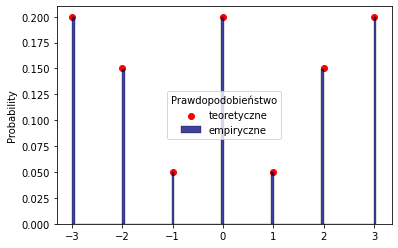
\includegraphics[scale=0.6]{dystrybuanta1.png}
			\caption{Rozkład prawdopodobieństwa}
		\end{center}
	\end{figure}
	
	\noindent Rozkład prawdopodobieństwa dla wygenerowanego wektora zmiennych losowych jest bardzo zbliżony do rozkładu teoretycznego.
	
	
	
	\subsection{Rozkład ciągły}	
	\noindent Algorytm:
	\begin{enumerate}
		\item Generujemy $U\sim U(0,1)$.
		\item Wstawiamy $X=F^{-1}_{X}\left( U \right) $. \\
	\end{enumerate}
	
	\noindent Chcemy wygenerować zmienne z rozkładu $ \mathrm{Exp} \left( \frac{1}{4} \right) $. Stwórzmy wektor długości $10^{5}$ zawierający zmienne losowe z rozkładu jednostajnego na przedziale $\left( 0,1 \right) $. Następnie odwracamy dystrybuantę $F_{X}$ i wstawiamy każdy element powyższego wektora jako argument otrzymanej funkcji.
	
	\begin{figure} [H]
		\centering 
		\subfigure[Histogram wektora zmiennych]{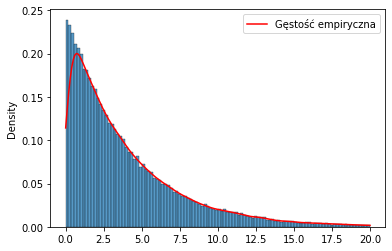
\includegraphics[scale=0.4877]{dystrybuanta2.png}}
		\subfigure[Najważniejsze statystyki opisowe]{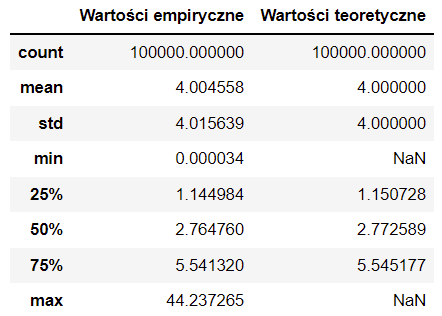
\includegraphics[scale=0.6477]{tabela_dystrybuanta.png}}
	\end{figure}
	
	\begin{figure} [H]
		\centering 
		\subfigure[Porównanie funkcji gęstości]{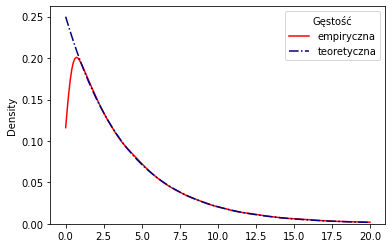
\includegraphics[scale=0.4877]{dystrybuanta3.png}}
		\subfigure[Porównanie dystrybuant]{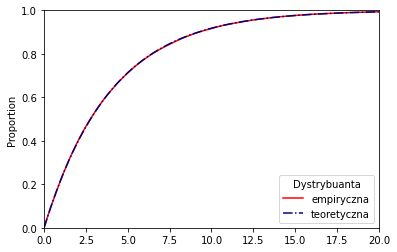
\includegraphics[scale=0.4877]{dystrybuanta4.png}}
	\end{figure}
	
	\begin{figure} [H]
		\centering 
		\subfigure[Wykres kwantylowy]{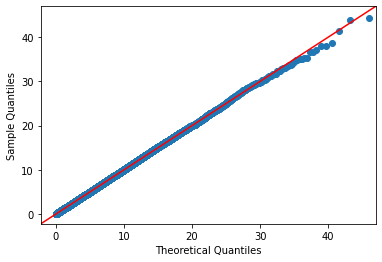
\includegraphics[scale=0.5]{dystrybuanta5.png}}
	\end{figure}
	
	\noindent Kształt histogramu odpowiada funkcji gęstości empirycznej. Wartości najważniejszych statystyk opisowych próby są zbliżone do wartości teoretycznych.
 Wykresy gęstości i dystrybuant się pokrywają, a wykres kwantylowy z argumentem $\mathrm{Exp} \left( \frac{1}{4} \right) $ stanowi linię prostą nachyloną do osi OX pod kątem $45$ stopni.
	
	
	\section{Metoda Boxa-Müllera}
	\noindent Służy do generowania zmiennych z rozkładu normalnego.
	$$X\sim N(\mu,\sigma) \hspace{2cm} f(x)=\dfrac{1}{\sigma\sqrt{2\pi}} \cdot \mathrm{exp}\left( -\dfrac{(x-\mu)^{2}}{2\sigma^{2}} \right)  $$
	
	\noindent Weźmy $X_{0}\sim N(0,1)$, wtedy $X \overset{\mathrm{d}}{=}\sigma X_{0} + \mu$. \\
	
	\noindent Algorytm:
	\begin{enumerate}
		\item Generujemy $U_{1}, U_{2}$ iid, $U_{i}\sim U(0,1)$.
		\item Wstawiamy
		$$X \overset{\mathrm{def}}{=} \sqrt{-2\ln{U_{1}}} \cdot \cos{\left( 2\pi U_{2} \right) }$$ 
		$$Y \overset{\mathrm{def}}{=} \sqrt{-2\ln{U_{1}}} \cdot \sin{\left( 2\pi U_{2} \right) }.$$
		Wtedy $X \upvDash Y$ oraz $X,Y \sim N(0,1)$. \\ \\
	\end{enumerate}
	
	\noindent Chcemy wygenerować zmienne z rozkładu $N(1,2)$.
	
	\begin{figure} [H]
		\centering 
		\subfigure[Histogram wektora zmiennych]{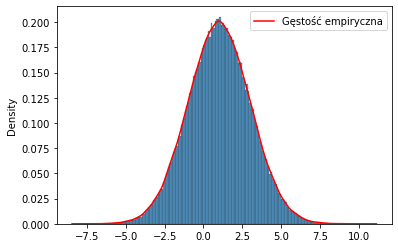
\includegraphics[scale=0.4877]{bm1.png}}
		\subfigure[Najważniejsze statystyki opisowe]{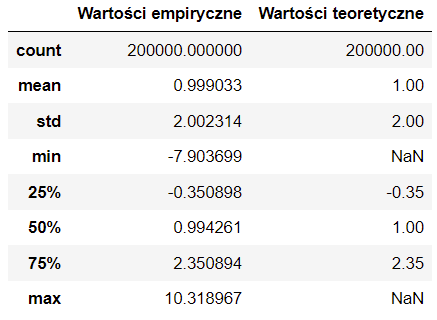
\includegraphics[scale=0.6475]{tabela_bm.png}}
	\end{figure}
	
	\begin{figure} [H]
		\centering 
		\subfigure[Porównanie funkcji gęstości]{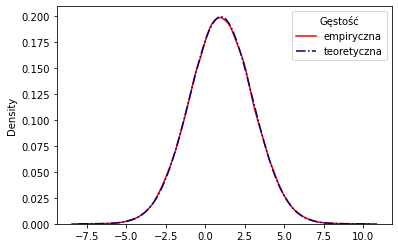
\includegraphics[scale=0.4865]{bm2.png}}
		\subfigure[Porównanie dystrybuant]{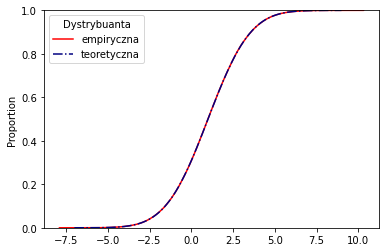
\includegraphics[scale=0.4865]{bm3.png}}
	\end{figure}
	
	\begin{figure} [H]
	\centering
	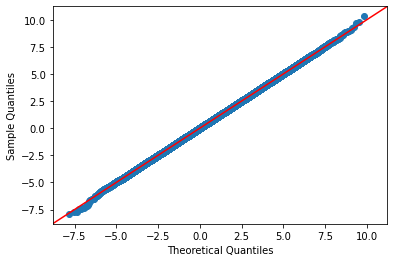
\includegraphics[scale=0.4877]{bm4.png}
	\end{figure}
	
	\noindent Kształt histogramu odpowiada funkcji gęstości empirycznej. Wartości najważniejszych statystyk opisowych próby są zbliżone do wartości teoretycznych.
 Wykresy gęstości i dystrybuant się pokrywają, a wykres kwantylowy z argumentem $N(1,2)$ stanowi linię prostą nachyloną do osi OX pod kątem 45 stopni.
	
	
	\section{Metoda biegunowa Boxa-Müllera}
	\noindent Metoda Boxa-Müllera jest mało wydajna. Obliczanie powyższych funkcji trygonometrycznych oparte jest na aproksymacji wielomianami. Możemy przekształcić tę metodę za pomocą współrzędnych biegunowych. \\ \\
	\noindent Załóżmy, że wektor losowy $\left( V_{1},V_{2} \right) $ ma rozkład jednostajny w kole jednostkowym.
	$R^{2} \rightarrow U_{1}$
	$$X \overset{\mathrm{def}}{=} \sqrt{-2\ln{U_{1}}} \cdot \cos{\left( 2\pi U_{2} \right) } \overset{\mathrm{d}}{=} \sqrt{-2\ln{R^{2}}} \cdot \cos{\left( \alpha \right) }  \overset{\mathrm{d}}{=} \sqrt{-2\ln{R^{2}}} \cdot \dfrac{V_{1}}{R} $$ 
	$$Y \overset{\mathrm{def}}{=} \sqrt{-2\ln{U_{1}}} \cdot \sin{\left( 2\pi U_{2} \right) \overset{\mathrm{d}}{=} \sqrt{-2\ln{R^{2}}} \cdot \sin{\left( \alpha \right) }  \overset{\mathrm{d}}{=} \sqrt{-2\ln{R^{2}}} \cdot \dfrac{V_{2}}{R}}.$$ \\
	
	\noindent Algorytm:
	\begin{enumerate}
		\item Generujemy $V_{1}, V_{2}$ iid, $V_{i } \sim U \left( -1,1 \right)$ .
		\item Wyznaczamy $R^{2}=V_{1}^{2} + V_{2}^{2}$.
		\item Jeśli $R^{2}>1$ to wracamy do $1$. 
		\item Wstawiamy
		$$X \overset{\mathrm{def}}{=} \sqrt{-2\ln{R^{2}}} \cdot \dfrac{V_{1}}{R}$$ 
		$$Y \overset{\mathrm{def}}{=} \sqrt{-2\ln{R^{2}}} \cdot \dfrac{V_{2}}{R}.$$
		Wtedy $X \upvDash Y$ oraz $X,Y \sim N(0,1)$. \\ \\
	\end{enumerate}
	
	\noindent Chcemy wygenerować zmienne z rozkładu $N(1,2)$.
	
	\begin{figure} [H]
		
		\centering 
		\subfigure[Histogram wektora zmiennych]{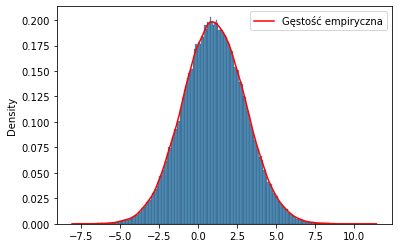
\includegraphics[scale=0.4877]{bmb1.png}}
		\subfigure[Najważniejsze statystyki opisowe]{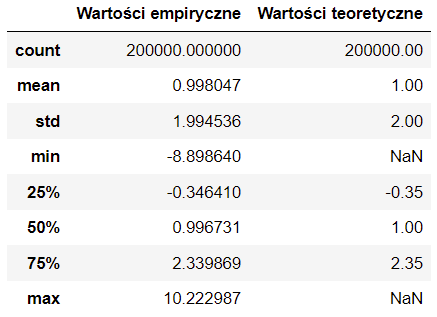
\includegraphics[scale=0.6477]{tabela_bmb.png}}
	\end{figure}	
	
	\begin{figure} [H]
		\centering 
		\subfigure[Porównanie funkcji gęstości]{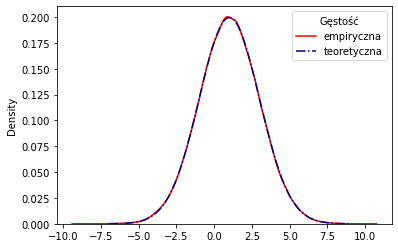
\includegraphics[scale=0.4877]{bmb2.png}}
		\subfigure[Porównanie dystrybuant]{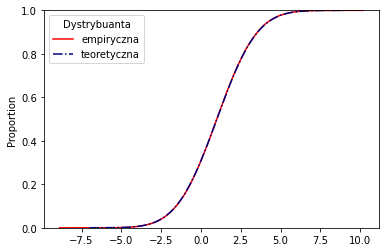
\includegraphics[scale=0.4877]{bmb3.png}}
	\end{figure}
	
	\begin{figure} [H]
		\centering 
		\subfigure[Wykres kwantylowy]{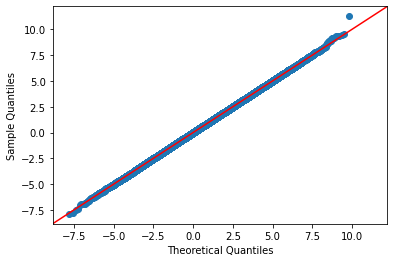
\includegraphics[scale=0.4877]{bmb4.png}}
	\end{figure}
	
	\noindent Kształt histogramu odpowiada funkcji gęstości empirycznej. Wartości najważniejszych statystyk opisowych próby są zbliżone do wartości teoretycznych.
 Wykresy gęstości i dystrybuant się pokrywają, a wykres kwantylowy z argumentem $N(1,2)$ stanowi linię prostą nachyloną do osi OX pod kątem 45 stopni.
 
 

	\section{Metoda akceptacji-odrzucenia}
	\noindent Metoda akceptacji-odrzucenia polega na generowania zmiennej losowej dyskretnej $X$ o rozkładzie
	$$p_i = P(X=i), i= 1,2, \ldots$$
	$$ \sum_{i} p_i = 1, p_1 \geqslant 0 $$.
	
	\subsection{Algorytm - rozkład dyskretny}
	\begin{enumerate}
	
	\item Generujemy jedną realizację $Y$.
	\item Generujemy $U \sim U(0,1)$ $U$ niezależne od $Y$.
	\item Jeśli $U \leqslant \frac{P_x}{cq_x}$ zwróć $X=Y$ w przeciwnym razie wróć do 1. \\ \\		
\end{enumerate}

\noindent Wykonaliśmy próbę dla $ P(X=1)=0.15, P(X=2) = 0.09, P(X=3)=0.04, P(X=4)=0.12, P(X=5)=0.18, P(X=6)=0.12, P(X=7)=0.04, P(X=8)=0.09, P(X=9) = 0,15$.
	
	\begin{figure}[H]
		\begin{center}
			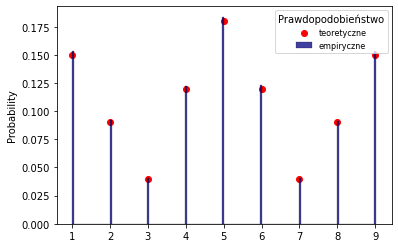
\includegraphics[scale=0.7]{ao1.png}
			\caption{Rozkład prawdopodobieństwa}
		\end{center}
	\end{figure}
	
	\noindent Rozkład prawdopodobieństwa dla wygenerowanego wektora zmiennych losowych jest bardzo zbliżony do rozkładu teoretycznego.
	
	\subsection{Algorytm - rozkłady ciągłe}
	\noindent Prawdopodobieństwo sukcesu pojedynczej iteracji algorytmu wynosi $\frac{1}{c}$. Liczba powtórzeń algorytmu ma rozkład $\mathrm{Geom}(\frac{1}{c})$. Średnia liczba powtórzeń algorytmu to $c$. \\ 
	
	\noindent Algorytm:	
	\begin{enumerate}
		\item Generujemy $U_1 \sim U(a,b)$ i $U_2 \sim U(O,m)$, $U_1$ niezależne od $U_2$.
		\item Jeśli $f(U_1) \geqslant U_2$ zwracamy $X=U_1$, w przeciwnym razie wróć do podpunktu 1. \\ 
	\end{enumerate}
	
	\noindent Wygenerowaliśmy próbę dla $f(x) = x^{3}$ oraz $g(x) = \sqrt[2]{\dfrac{1}{2}}$.

		\begin{figure}[H]
		\begin{center}
			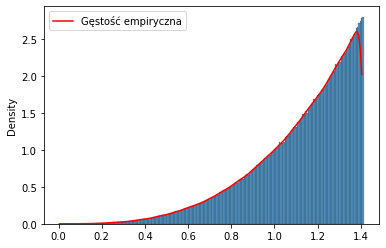
\includegraphics[scale=0.7]{ao2.png}
			\caption{Histogram wektora zmiennych}
		\end{center}
	\end{figure}
	
	
		\begin{figure} [H]
			\centering 
			\subfigure[Porównanie funkcji gęstości]{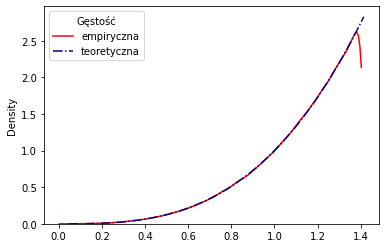
\includegraphics[scale=0.4877]{ao3.png}}
			\subfigure[Porównanie dystrybuant]{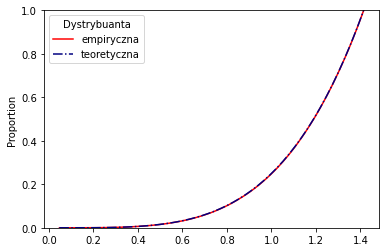
\includegraphics[scale=0.4877]{ao4.png}}
		\end{figure}
	
	
	
 	\noindent Kształt histogramu odpowiada funkcji gęstości empirycznej, a wykresy gęstości i dystrybuant się pokrywają.
   
 	\section{Metoda splotowa}
 	\noindent Metoda ta pozwala wygenerować pewną zmienną losową $X$, przy pomocy innych zmiennych, które potrafimy efektywnie generować, i zsumowaniu ich. Załóżmy, że
 	$$ X \buildrel{d} \over{=} Y_1 + Y_2 + \dots + Y_n, $$
 	gdzie $Y_i$ to zmienne losowe niezależne. 
 	
 	
 	\subsection{Algorytm - rozkład dyskretny}
 	\begin{enumerate}
 		\item Generujemy $U_1, \ldots, U_n$, iid. $U_1 \sim (0,1)$
 		\item Wstaw $ X = (U_1 \leqslant p) + \ldots + (U_n \leqslant p)$ \\ 
 	\end{enumerate} 
 	
 	\noindent Aby zobaczyć wyniki działań skorzystaliśmy z rozkładu Bernoulliego. 
 	
 	\begin{figure}[H]
 	\begin{center}
 		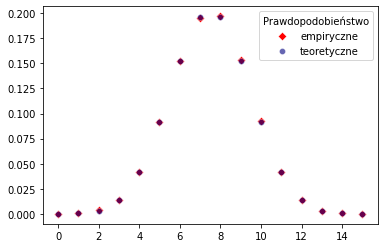
\includegraphics[scale=0.6]{splot1.png}
 		\caption{Prawdopodobieństwo zmiennych losowych}
 	\end{center}
 	\end{figure}
 
 	\subsection{Algorytm - rozkład ciągły}
 	\begin{enumerate}
 		\item Generujemy $ Y_1, Y_2, \dots, Y_n $.
 		\item Zwracamy $ X = Y_1 + Y_2 + \dots + Y_n $. \\ \\
 	\end{enumerate}
 	
 	\noindent Nasze wyniki zostały uzyskane za pomocą rozkładu chi-kwadrat, $X_i  \sim N(0,1)$, o $3$ stopniach swobody.
 	
 	\begin{figure} [H]
 		\centering 
 		\subfigure[Histogram wektora zmiennych]{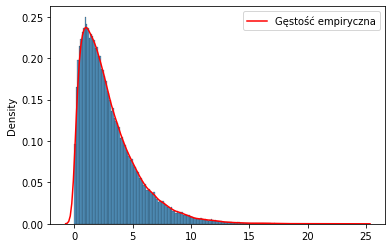
\includegraphics[scale=0.4877]{splot2.png}}
 		\subfigure[Porównanie funkcji gęstości]{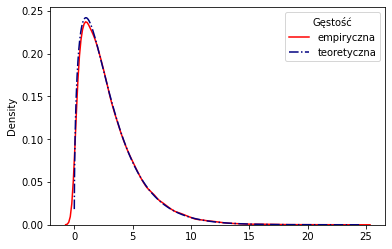
\includegraphics[scale=0.4877]{splot3.png}}
 	\end{figure}
 	\begin{figure} [H]
 		\centering 
 		\subfigure[Porównanie dystrybuant]{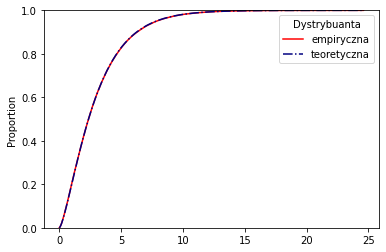
\includegraphics[scale=0.4877]{splot4.png}}
 		\subfigure[Wykres kwantylowy]{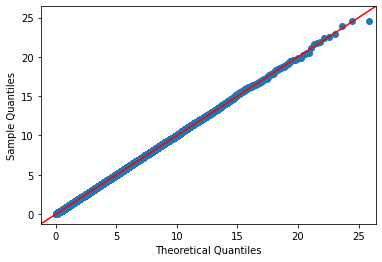
\includegraphics[scale=0.4877]{splot5.png}}
 	\end{figure}
 
 
  	\noindent Kształt histogramu odpowiada funkcji gęstości empirycznej. Wykresy gęstości i dystrybuant się pokrywają, a wykres kwantylowy z argumentem $\mathrm{chi}^{2}(3)$ stanowi linię prostą nachyloną do osi OX pod kątem 45 stopni.
 
 
 	\section{Metoda kompozycji}
 	\noindent Załóżmy, że $X$ ma dystrybuantę postaci $F_x (x) = \sum_{i=1}^{n} p_i F_i (x)$, gdzie $p_i > 0$, $\sum_{i=1}^{n} p_i = 1$ oraz $F_i$ to dystrybunaty pewnych zmiennych losowych $Y_i$.
 	
 	\subsection{Algorytm - metoda kompozycji}
 	\begin{enumerate}
 		\item Generujemy zmienną losową $I$ o rozkładzie $P(I=i)=p_i, \quad i = 1,2,...,n$ $ \quad I \upvDash Y_i$.
 		\item Generujemy zmienną losową $Y_I$.
 		\item Wstaw $X=Y_I$. \\ \\
 	\end{enumerate}
 	
	\noindent Wykonaliśmy metodę dla rozkładu ciągłego dla rozkładu ciągłego Laplace’a z parametrem $\lambda = \frac{1}{b}$, gdzie $b = 1$. 	
 	
 	\begin{figure} [H]
 	\centering 
 	\subfigure[Histogram wektora zmiennych]{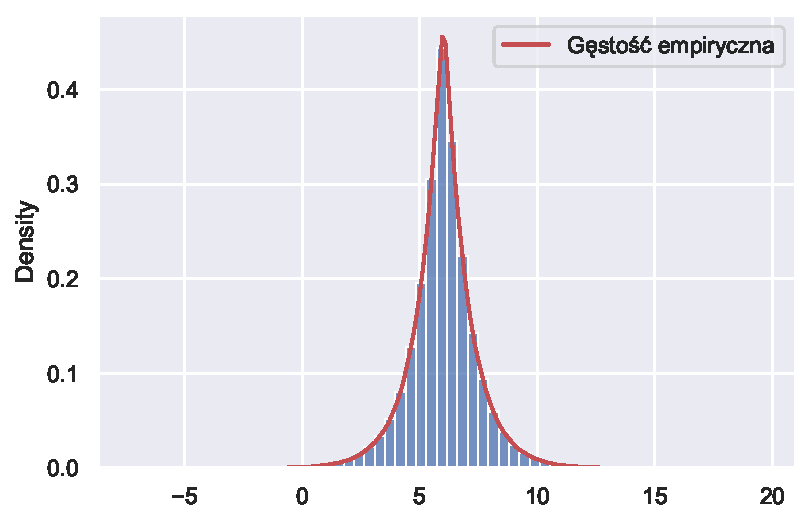
\includegraphics[scale=0.4685]{kompozycja1.pdf}}
    	\subfigure[Porównanie funkcji gęstości]{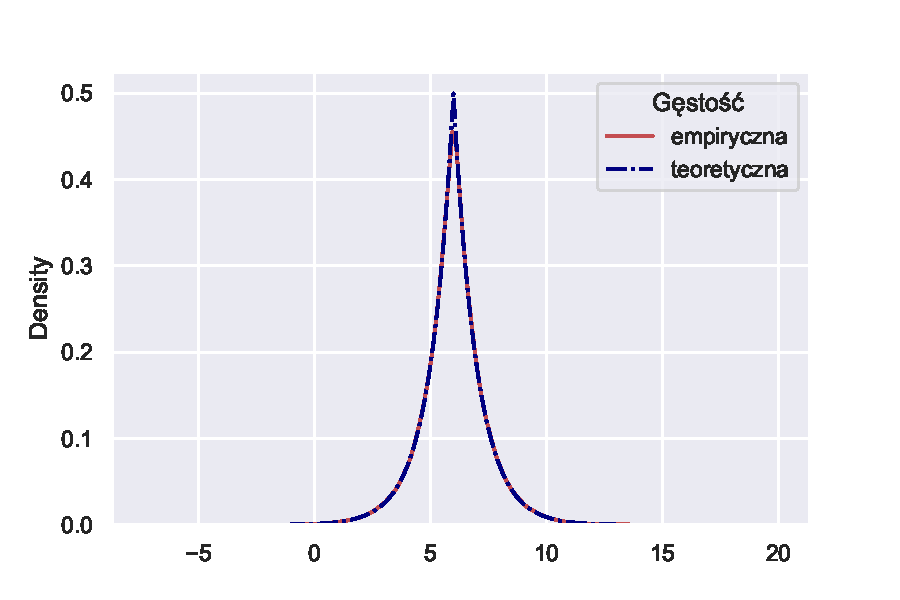
\includegraphics[scale=0.4685]{kompozycja2.pdf}}
 	\end{figure}
 
 	
 	
 	 	\noindent Kształt histogramu odpowiada funkcji gęstości empirycznej, a wykresy gęstości  się pokrywają.
 	
 
 	
 	\section{Liniowy generator kongruentny}
 	\noindent
 	Liczba losowa jest, to liczba $r$  należącą do pewnego zbioru wartości ${r_1, ..., r_n}$ wybieranych z pewnym prawdopodobieństwem, z kolei liczby pseudolosowe wyglądają jak losowe, lecz tworzy się je algorytmicznie. Oznacza to, iż znając wzór generacyjny oraz kilka kolejnych liczb pseudolosowych możemy bez problemu wygenerować wszystkie dalsze - tej cechy nie posiadają liczby losowe, w przeciwnym razie totolotek straciłby sens.
 	
 	\noindent Liniowy generator kongruentny zaproponowany przez D. H. Lehmera w 1951 roku. Większość dzisiejszych procedur do generowania liczb pseudolosowych jest oparta na tym generatorze. 
 	$$x_{n+1} =(ax_n + b)(\mathrm{mod} \quad m)$$ 
 	
 	\noindent Zwykle wybieramy $m$ najbliższe największej liczbie całkowitej dostępnej dla komputera.
 	
 	\begin{figure} [H]
 		\centering 
 		\subfigure[Histogram wektora zmiennych]{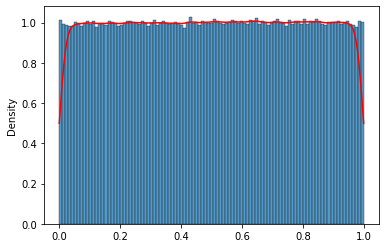
\includegraphics[scale=0.4877]{lcg1.png}}
 		\subfigure[Porównanie funkcji gęstości]{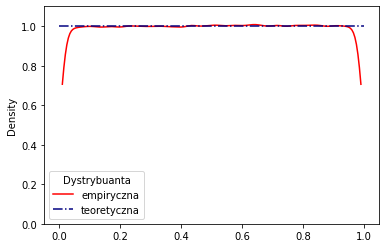
\includegraphics[scale=0.4877]{lcg2.png}}
 	\end{figure}
    \begin{figure} [H]
    	\centering 
    	\subfigure[Porównanie dystrybuant]{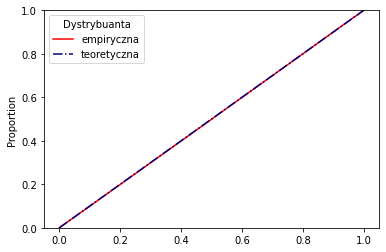
\includegraphics[scale=0.4877]{lcg3.png}}
    	\subfigure[Wykres kwantylowy]{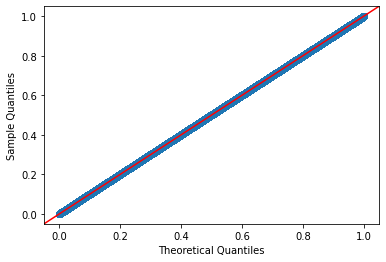
\includegraphics[scale=0.4867]{lcg4.png}}
    \end{figure}
    
    \noindent Kształt histogramu odpowiada funkcji gęstości empirycznej. Wykresy gęstości i dystrybuant się pokrywają, a wykres kwantylowy z argumentem $U \left( 0,1 \right) $ stanowi linię prostą nachyloną do osi OX pod kątem $45$ stopni.
   
   \section{Wnioski}
   \noindent Za pomocą wyżej wymienionych metod jesteśmy w stanie efektywnie generować realizacje zmiennych losowych o różnych rozkładach. Pozwalają nam one w pewien sposób "obejść" praktyczną niemożność komputera do wykonywania operacji prawdziwie losowych. Wykresy dystrybuant, gęstości oraz wartości statystyk opisowych dla danych rozkładów możemy wysymulować na tyle dokładnie, ażeby móc wykorzystywać potencjał komputera do obliczeń, w których korzystamy z teorii rachunku prawdopodobieństwa.
 

\end{document}
